% Options for packages loaded elsewhere
\PassOptionsToPackage{unicode}{hyperref}
\PassOptionsToPackage{hyphens}{url}
\PassOptionsToPackage{dvipsnames,svgnames,x11names}{xcolor}
%
\documentclass[
  12pt]{article}

\usepackage{amsmath,amssymb}
\usepackage{iftex}
\ifPDFTeX
  \usepackage[T1]{fontenc}
  \usepackage[utf8]{inputenc}
  \usepackage{textcomp} % provide euro and other symbols
\else % if luatex or xetex
  \usepackage{unicode-math}
  \defaultfontfeatures{Scale=MatchLowercase}
  \defaultfontfeatures[\rmfamily]{Ligatures=TeX,Scale=1}
\fi
\usepackage{lmodern}
\ifPDFTeX\else  
    % xetex/luatex font selection
\fi
% Use upquote if available, for straight quotes in verbatim environments
\IfFileExists{upquote.sty}{\usepackage{upquote}}{}
\IfFileExists{microtype.sty}{% use microtype if available
  \usepackage[]{microtype}
  \UseMicrotypeSet[protrusion]{basicmath} % disable protrusion for tt fonts
}{}
\makeatletter
\@ifundefined{KOMAClassName}{% if non-KOMA class
  \IfFileExists{parskip.sty}{%
    \usepackage{parskip}
  }{% else
    \setlength{\parindent}{0pt}
    \setlength{\parskip}{6pt plus 2pt minus 1pt}}
}{% if KOMA class
  \KOMAoptions{parskip=half}}
\makeatother
\usepackage{xcolor}
\setlength{\emergencystretch}{3em} % prevent overfull lines
\setcounter{secnumdepth}{5}
% Make \paragraph and \subparagraph free-standing
\makeatletter
\ifx\paragraph\undefined\else
  \let\oldparagraph\paragraph
  \renewcommand{\paragraph}{
    \@ifstar
      \xxxParagraphStar
      \xxxParagraphNoStar
  }
  \newcommand{\xxxParagraphStar}[1]{\oldparagraph*{#1}\mbox{}}
  \newcommand{\xxxParagraphNoStar}[1]{\oldparagraph{#1}\mbox{}}
\fi
\ifx\subparagraph\undefined\else
  \let\oldsubparagraph\subparagraph
  \renewcommand{\subparagraph}{
    \@ifstar
      \xxxSubParagraphStar
      \xxxSubParagraphNoStar
  }
  \newcommand{\xxxSubParagraphStar}[1]{\oldsubparagraph*{#1}\mbox{}}
  \newcommand{\xxxSubParagraphNoStar}[1]{\oldsubparagraph{#1}\mbox{}}
\fi
\makeatother


\providecommand{\tightlist}{%
  \setlength{\itemsep}{0pt}\setlength{\parskip}{0pt}}\usepackage{longtable,booktabs,array}
\usepackage{calc} % for calculating minipage widths
% Correct order of tables after \paragraph or \subparagraph
\usepackage{etoolbox}
\makeatletter
\patchcmd\longtable{\par}{\if@noskipsec\mbox{}\fi\par}{}{}
\makeatother
% Allow footnotes in longtable head/foot
\IfFileExists{footnotehyper.sty}{\usepackage{footnotehyper}}{\usepackage{footnote}}
\makesavenoteenv{longtable}
\usepackage{graphicx}
\makeatletter
\def\maxwidth{\ifdim\Gin@nat@width>\linewidth\linewidth\else\Gin@nat@width\fi}
\def\maxheight{\ifdim\Gin@nat@height>\textheight\textheight\else\Gin@nat@height\fi}
\makeatother
% Scale images if necessary, so that they will not overflow the page
% margins by default, and it is still possible to overwrite the defaults
% using explicit options in \includegraphics[width, height, ...]{}
\setkeys{Gin}{width=\maxwidth,height=\maxheight,keepaspectratio}
% Set default figure placement to htbp
\makeatletter
\def\fps@figure{htbp}
\makeatother

\addtolength{\oddsidemargin}{-.5in}%
\addtolength{\evensidemargin}{-1in}%
\addtolength{\textwidth}{1in}%
\addtolength{\textheight}{1.7in}%
\addtolength{\topmargin}{-1in}%
\usepackage{booktabs}
\usepackage{longtable}
\usepackage{array}
\usepackage{multirow}
\usepackage{wrapfig}
\usepackage{float}
\usepackage{colortbl}
\usepackage{pdflscape}
\usepackage{tabu}
\usepackage{threeparttable}
\usepackage{threeparttablex}
\usepackage[normalem]{ulem}
\usepackage{makecell}
\usepackage{xcolor}
\usepackage{amsmath}
\usepackage{float}
\usepackage{hyperref}
\usepackage[utf8]{inputenc}
\usepackage{bm}
\def\tightlist{}
\usepackage{setspace}
\newcommand\pD{$p\text{-}D$}
\newcommand\kD{$k\text{-}D$}
\newcommand\dD{$d\text{-}D$}
\newcommand\gD{$2\text{-}D$}
\makeatletter
\@ifpackageloaded{caption}{}{\usepackage{caption}}
\AtBeginDocument{%
\ifdefined\contentsname
  \renewcommand*\contentsname{Table of contents}
\else
  \newcommand\contentsname{Table of contents}
\fi
\ifdefined\listfigurename
  \renewcommand*\listfigurename{List of Figures}
\else
  \newcommand\listfigurename{List of Figures}
\fi
\ifdefined\listtablename
  \renewcommand*\listtablename{List of Tables}
\else
  \newcommand\listtablename{List of Tables}
\fi
\ifdefined\figurename
  \renewcommand*\figurename{Figure}
\else
  \newcommand\figurename{Figure}
\fi
\ifdefined\tablename
  \renewcommand*\tablename{Table}
\else
  \newcommand\tablename{Table}
\fi
}
\@ifpackageloaded{float}{}{\usepackage{float}}
\floatstyle{ruled}
\@ifundefined{c@chapter}{\newfloat{codelisting}{h}{lop}}{\newfloat{codelisting}{h}{lop}[chapter]}
\floatname{codelisting}{Listing}
\newcommand*\listoflistings{\listof{codelisting}{List of Listings}}
\makeatother
\makeatletter
\makeatother
\makeatletter
\@ifpackageloaded{caption}{}{\usepackage{caption}}
\@ifpackageloaded{subcaption}{}{\usepackage{subcaption}}
\makeatother

\ifLuaTeX
  \usepackage{selnolig}  % disable illegal ligatures
\fi
\usepackage[]{natbib}
\bibliographystyle{agsm}
\usepackage{bookmark}

\IfFileExists{xurl.sty}{\usepackage{xurl}}{} % add URL line breaks if available
\urlstyle{same} % disable monospaced font for URLs
\hypersetup{
  pdftitle={Looking at Non-Linear Dimension Reductions as Models in the Data Space},
  pdfauthor={Jayani P.G. Lakshika; Dianne Cook; Paul Harrison; Michael Lydeamore; Thiyanga S. Talagala},
  pdfkeywords={high-dimensional data vizualization, non-linear dimension
reduction, tour},
  colorlinks=true,
  linkcolor={blue},
  filecolor={Maroon},
  citecolor={Blue},
  urlcolor={Blue},
  pdfcreator={LaTeX via pandoc}}



\begin{document}


\def\spacingset#1{\renewcommand{\baselinestretch}%
{#1}\small\normalsize} \spacingset{1}


%%%%%%%%%%%%%%%%%%%%%%%%%%%%%%%%%%%%%%%%%%%%%%%%%%%%%%%%%%%%%%%%%%%%%%%%%%%%%%

\title{\bf Looking at Non-Linear Dimension Reductions as Models in the
Data Space}
\author{
Jayani P.G. Lakshika\\
Econometrics \& Business Statistics, Monash University\\
and\\Dianne Cook\\
Econometrics \& Business Statistics, Monash University\\
and\\Paul Harrison\\
MGBP, BDInstitute, Monash University\\
and\\Michael Lydeamore\\
Econometrics \& Business Statistics, Monash University\\
and\\Thiyanga S. Talagala\\
Statistics, University of Sri Jayewardenepura\\
}
\maketitle

\bigskip
\bigskip
\begin{abstract}
Non-linear dimension reduction (NLDR) techniques such as tSNE, and UMAP
provide a low-dimensional representation of high-dimensional data
(\pD{}) by applying a non-linear transformation. NLDR often exaggerates
random patterns, sometimes due to the samples observed. But NLDR views
have an important role in data analysis because, if done well, they
provide a concise visual (and conceptual) summary of \pD{}
distributions. The NLDR methods and (hyper)parameter choices can create
wildly different representations, making it difficult to decide which is
best, or whether any or all are accurate or misleading. To help assess
the NLDR and decide on which, if any, is the most reasonable
representation of the structure(s) present in the \pD{} data, we have
developed an algorithm to show the \gD{} NLDR model in the \pD{} space,
viewed with a tour, a movie of linear projections. From this, one can
see if the model fits everywhere, or better in some subspaces, or
completely mismatches the data. Also, we can see how different methods
may have similar summaries or quirks.
\end{abstract}

\noindent%
{\it Keywords:} high-dimensional data vizualization, non-linear
dimension reduction, tour
\vfill

\newpage
\spacingset{1.9} % DON'T change the spacing!


\spacingset{1.0}

\section{Introduction}\label{introduction}

Non-linear dimension reduction (NLDR) is popular for making a convenient
low-dimensional (\kD{}) representation of high-dimensional (\pD{}) data
(\(k < p\)). Recently developed methods include t-distributed stochastic
neighbor embedding (tSNE) \citep{laurens2008}, uniform manifold
approximation and projection (UMAP) \citep{leland2018}, potential of
heat-diffusion for affinity-based trajectory embedding (PHATE) algorithm
\citep{moon2019}, large-scale dimensionality reduction Using triplets
(TriMAP) \citep{amid2022}, and pairwise controlled manifold
approximation (PaCMAP) \citep{yingfan2021}. However, the representation
generated can vary dramatically from method to method, and with
different choices of parameters or random seeds made using the same
method (Figure~\ref{fig-NLDR-variety}). The dilemma for the analyst is
then, \textbf{which representation to use}. The choice might result in
different procedures used in the downstream analysis, or different
inferential conclusions. The research described here provides new visual
tools to aid with this decision.

\begin{figure}

\centering{

\includegraphics[width=1\textwidth,height=\textheight]{paper_files/figure-pdf/fig-NLDR-variety-1.pdf}

}

\caption{\label{fig-NLDR-variety}Eight different NLDR representations of
the same data. Different techniques and different parameter choices are
used. Researchers may have seen any of these in their analysis of this
data, depending on their choice of method, or typical parameter choice.
Would they make different decisions downstream in the analysis depending
on which version seen? Which is the most accurate representation of the
structure in high dimensions?}

\end{figure}%

The paper is organized as follows. Section~\ref{sec-background} provides
a summary of the literature on NLDR, and high-dimensional data
visualization methods. Section~\ref{sec-method} contains the details of
the new methodology, including simulated data examples. Two applications
illustrating the use of the new methodology for bioinformatics and image
classification are in Section~\ref{sec-applications}. Limitations and
future directions are provided in Section~\ref{sec-discussion}.

\section{Background}\label{sec-background}

Historically, \kD{} representations of \pD{} data have been computed
using multidimensional scaling (MDS) \citep{borg2005}, which includes
principal components analysis (PCA) \citep{jolliffe2011} as a special
case. The \kD{} representation can be considered to be a layout of
points in \kD{} produced by an embedding procedure that maps the data
from \pD{}. In MDS, the \kD{} layout is constructed by minimizing a
stress function that differences distances between points in \pD{} with
potential distances between points in \kD{}. Various formulations of the
stress function result in non-metric scaling \citep{saeed2018} and
isomap \citep{silva2002}. Challenges in working with high-dimensional
data, including visualization, are outlined in \citet{johnstone2009}.

Many new methods for NLDR have emerged in recent years, all designed to
better capture specific structures potentially existing in \pD{}. Here
we focus on five currently popular techniques, tSNE, UMAP, PHATE, TriMAP
and PaCMAP. tNSE and UMAP can be considered to produce the \kD{}
minimizing the divergence between two distributions, where the
distributions are modeling the inter-point distances. PHATE, TriMAP and
PaCMAP are examples of diffusion processes \citep{coifman2005} spreading
to capture geometric shapes, that include both global and local
structure.

The array of layouts in Figure~\ref{fig-NLDR-variety} illustrate what
can emerge from the choices of method and parameters, and the random
seed that initiates the computation. Key structures interpreted from
these views suggest: (1) highly \textbf{separated clusters} (a, b, e, g,
h) with the number ranging from 3-6; (2) \textbf{stringy branches} (f),
and (3) \textbf{barely separated clusters} (c, d) which would
\textbf{contradict} the other representations.

It happens because these methods and parameter choices provide different
lenses on the interpoint distances in the data.

The alternative approach to visualizing the high-dimensional data is to
use linear projections. PCA is the classical approach, resulting in a
set of new variables which are linear combinations of the original
variables. Tours, defined by \citet{lee2021}, broaden the scope by
providing movies of linear projections, that provide views the data from
all directions. \citet{lee2021} provides an review of the main
developments in tours. There are many tour algorithms implemented, with
many available in the R package \texttt{tourr} \citep{wickham2011}, and
versions enabling better interactivity in \texttt{langevitour}
\citep{harisson2024} and \texttt{detourr} \citep{hart2022}. Linear
projections are a safe way to view high-dimensional data, because they
do not warp the space, so they are more faithful representations of the
structure. However, linear projections can be cluttered, and global
patterns can obscure local structure. The simple activity of projecting
data from \pD{} suffers from piling \citep{laa2022}, where data
concentrates in the center of projections. NLDR is designed to escape
these issues, to exaggerate structure so that it can be observed. But as
a result NLDR can hallucinate wildly, to suggest patterns that are not
actually present in the data.

The solution is to use the tour to examine how the NLDR is warping the
space. This approach follows what \citet{wickham2015} describes as
\emph{model-in-the-data-space}. The fitted model should be overlaid on
the data, to examine the fit relative the spread of the observations.
While this is straightforward, and commonly done when data is \gD{}, it
is also possible in \pD{}, for many models, when a tour is used.

\citet{wickham2015} provides several examples of models overlaid on the
data in \pD{}. In hierarchical clustering, a representation of the
dendrogrom using points and lines can be constructed by augmenting the
data with points marking merging of clusters. Showing the movie of
linear projections reveals shows how the algorithm sequentially fitted
the cluster model to the data. For linear discriminant analysis or
model-based clustering the model can be indicated by \((p-1)\text{-}D\)
ellipses. It is possible to see whether the elliptical shapes
appropriately matches the variance of the relevant clusters, and to
compare and contrast different fits. For PCA, one can display the \kD{}
plane of the reduced dimension using wireframes of transformed cubes.
Using a wireframe is the approach we take here, to represent the NLDR
model in \pD{}.

\section{Method}\label{sec-method}

\subsection{What is the NLDR model?}\label{what-is-the-nldr-model}

At first glance, thinking of NLDR as a modeling technique might seem
strange. It is a simplified representation or abstraction of a system,
process, or phenomenon in the real world. The \pD{} observations are the
realization of the phenomenon, and the \kD{} NLDR layout is the
simplified representation. From a statistical perspective we can
consider the distances between points in the \kD{} layout to be variance
that the model explains, and the (relative) difference with their
distances in \pD{} is the error, or unexplained variance. We can also
imagine that the positioning of points in \gD{} represent the fitted
values, that will have some prescribed position in \pD{} that can be
compared with their observed values. This is the conceptual framework
underlying the more formal versions of factor analysis \citep{cfa69} and
multidimensional scaling (MDS) \citep{borg2005}. (Note that, for this
thinking the full \pD{} data needs to be available, not just the
interpoint distances.)

\begin{table}

\centering{

\centering\begingroup\fontsize{12}{14}\selectfont

\begin{tabular}{>{\raggedright\arraybackslash}p{3cm}>{\raggedright\arraybackslash}p{12cm}}
\toprule
\textbf{Notation} & \textbf{Description}\\
\midrule
$n, p, k$ & number of observations, variables, embedding dimension, respectively\\
$\mathbfit{X}, \mathbfit{x}$ & $p$-dimensional data (population, sample)\\
$\mathbfit{y}$ & $k$-dimensional layout\\
$P$ & orthonormal basis, generating a $d\text{-}dimensional$ linear projection of $p$-dimensional data\\
$T$ & true  model\\
\addlinespace
$g$ & functional mapping from \pD{} to \kD{}, especially as prescribed by NLDR\\
$\mathbfit{\theta}$ & (Hyper-) parameters for NLDR method\\
$r$ & ranges of the embedding components\\
$C^{(j)}$ & $j$-dimensional bin centers\\
$(b_1, b_2)$ & number of bins in each direction\\
\addlinespace
$(a_1, a_2)$ & binwidths, distance between centroids in each direction\\
$(s_1, \ s_2)$ & starting coordinates of the hexagonal grid\\
$q$ & buffer to ensure hexgrid covers data, proportion of data range, 0-1\\
$m$ & number of non-empty bins\\
$b$ & number of  hexagons in the grid\\
\addlinespace
$h$ & hexagonal id\\
$l$ & side length\\
$A$ & area\\
\bottomrule
\end{tabular}
\endgroup{}

}

\caption{\label{tbl-notation}Summary of notation for describing new
methodology.}

\end{table}%

We define the NLDR as a function
\(g\text{:}~ \mathbb{R}^{n\times p} \rightarrow \mathbb{R}^{n\times k}\),
with (hyper-)parameters \(\mathbfit{\theta}\). The parameters,
\(\mathbfit{\theta}\), depend on the choice of \(g\), and can be
considered part of model fitting in the traditional sense. Common
choices for \(g\) include functions used in tSNE, UMAP, PHATE, TriMAP,
PaCMAP, or MDS, although in theory any function that does this mapping
is suitable.

With our goal being to make a representation of this \gD{} layout that
can be lifted into high-dimensional space, the layout needs to be
augmented to include neighbour information. A simple approach would be
to triangulate the points and add edges. A more stable approach is to
first bin the data, reducing it from \(n\) to \(m\leq n\) observations,
and connect the bin centroids. We recommend using a hexagon grid because
it better reflects the data distribution and has less artifacts than a
rectangular grid. This process serves to reduce some noisiness in the
resulting surface shown in \pD{}. The steps in this process are shown in
Figure~\ref{fig-NLDR-two-curvy}, and documented below.

To illustrate the method, we use \(7\text{-}D\) simulated data, which we
call the ``S-curve''. It is constructed by simulating \(n=750\)
observations from \(\theta \sim U(-3\pi/2, 3\pi/2)\),
\(X_1 = \sin(\theta)\), \(X_2 \sim U(0, 2)\) (adding thickness to the
S), \(X_3 = \text{sign}(\theta) \times (\cos(\theta) - 1)\). The
remaining variables \(X_4, X_5, X_6, X_7\) are all uniform error, with
small variance. We would consider \(T=(X_1, X_2, X_3)\) to be the
geometric structure (true model) that we hope to capture.

\begin{figure}[H]

\centering{

\includegraphics[width=1\textwidth,height=\textheight]{paper_files/figure-pdf/fig-two-curvy-true-proj-1.pdf}

}

\caption{\label{fig-two-curvy-true-proj}Two views of the true model
(blue lines) in \(2\text{-}D\) projections from \(7\text{-}D\), for the
two C-shaped clusters data (grey points). In one C-shaped cluster, the
data is spread throughout the cluster, while in the other C-shaped
cluster, the data is concentrated more in one corner of the cluster. The
\textbf{langevitour} software is used to view the data with a tour, and
the full video is available at \textless\textgreater.}

\end{figure}%

\begin{figure}

\centering{

\includegraphics[width=1\textwidth,height=\textheight]{paper_files/figure-pdf/fig-NLDR-two-curvy-1.pdf}

}

\caption{\label{fig-NLDR-two-curvy}Key steps for constructing the model
on the UMAP layout (\(k=2\)): (a) data, (b) hexagon bins, (c) bin
centroids, and (d) triangulated centroids. The two C-shaped clusters
data is shown.}

\end{figure}%

\subsection{\texorpdfstring{Algorithm to represent the model in
\gD{}}{Algorithm to represent the model in }}\label{algorithm-to-represent-the-model-in}

\subsubsection{Scale the data}\label{scale-the-data}

Because we are working with distances between points, starting with data
having a standard scale, e.g.~{[}0, 1{]}, is recommended. The default
should take the aspect ratio produced by the NLDR
\((r_1, r_2, ..., r_k)\) into account. When \(k=2\), as in hexagon
binning, the default range is \([0, y_{i,\text{max}}], i=1,2\), where
\(y_{1,\text{max}}=1\) and \(y_{2,\text{max}} = \frac{r_2}{r_1}\)
(Figure~\ref{fig-NLDR-two-curvy}). If the NLDR aspect ratio is ignored
then set \(y_ {2,\text{max}} = 1\).

\subsubsection{Computing hexagon grid
configuration}\label{computing-hexagon-grid-configuration}

Although there are several implementations of hexagon binning
\citep{carr1987}, and a published paper \citep{dan2023}, surprisingly,
none has sufficient detail or components that produce everything needed
for this project. So we described the process used here.
Figure~\ref{fig-hex-param} illustrates the notation used.

The \gD{} hexagon grid is defined by its bin centroids. Each hexagon,
\(H_h\) (\(h = 1, \dots, b\)) is uniquely described by centroid,
\(C_{h}^{(2)} = (c_{h1}, c_{h2})\). The number of bins in each direction
is denoted as \((b_1, b_2)\), with \(b = b_1 \times b_2\) being the
total number of bins. We expect the user to provide just \(b_1\) and we
calculate \(b_2\) using the NLDR ratio, to compute the grid.

To ensure that the grid covers the range of data values a buffer
parameter (\(q\)) is set as a proportion of the range. By default,
\(q=0.1\). The buffer should be extending a full hexagon width (\(a_1\))
and height (\(a_2\)) beyond the data, in all directions. The lower left
position where the grid starts is defined as \((s_1, s_2)\), and
corresponds to the centroid of the lowest left hexagon,
\(C_{1}^{(2)} = (c_{11}, c_{12})\). This must be smaller than the
minimum data value. Because it is one buffer unit, \(q\) below the
minimum data values, \(s_1 = -q\) and \(s_2 = -qr_2\).

The value for \(b_2\) is computed by fixing \(b_1\). Considering the
upper bound of the first NLDR component, \(a_1 > \frac{1+2q}{b_1 -1}\).
Similarly, for the second NLDR component,
\(a_2 > \frac{r_2 + q(1 + r_2)}{(b_2 - 1)}\). Since
\(a_2 = \frac{\sqrt(3)}{2}a_1\) for regular hexagons,
\(a_1 > \frac{2[r_2 + q(1 + r_2)]}{\sqrt{3}(b_2 - 1)}\). This is a
linear optimization problem. Therefore, the optimal solution must occur
on a vertex. Therefore,
\(b_2 = \Big\lceil1 +\frac{2[r_2 + q(1 + r_2)](b_1 - 1)}{\sqrt{3}(1 + 2q)}\Big\rceil\).

\begin{figure}[H]

\centering{

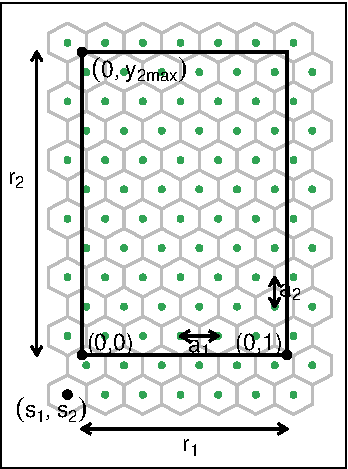
\includegraphics[width=0.3\textwidth,height=\textheight]{paper_files/figure-pdf/fig-hex-param-1.pdf}

}

\caption{\label{fig-hex-param}The components of the hexagon grid
illustrating notation.}

\end{figure}%

\subsubsection{Binning the data}\label{binning-the-data}

Observations are grouped into bins based on their nearest centroid. This
produces a reduction in size of the data from \(n\) to \(m\), where
\(m\leq b\) (total number of bins). This can be defined using the
function
\(u: \mathbb{R}^{n\times 2} \rightarrow \mathbb{R}^{m\times 2}\), where
\(u(i) = \arg\min_{j = 1, \dots, b} \sqrt{(y_{i1} - C^{(2)}_{j1})^2 + (y_{i2} - C^{(2)}_{j2})^2}\),
mapping observation \(i\) into \(H_h = \{i| u(i) = h\}\).

By default, the bin centroid is used for describing a hexagon (as done
in Figure~\ref{fig-NLDR-two-curvy} (c)), but any measure of center, such
as a mean or weighted mean of the points within each hexagon, could be
used. The bin centers, and the binned data, are the two important
components needed to render the model representation in high dimensions.

\subsubsection{Indicating neighborhood}\label{indicating-neighborhood}

Delaunay triangulation \citep{lee1980, alb2024} is used to connect
points so that edges indicate neighbouring observations, in both the
NLDR layout (Figure~\ref{fig-NLDR-two-curvy} (d)) and the \pD{} model
representation. When the data has been binned the triangulation connectd
centroids. The edges preserve the neighborhood information when the
model is lifted into \pD{}.

When shapes are non-linear in the NLDR layout, some edges could be long.
It can also happen that distant centroids can be connected, particularly
if clustering is present, which can result in long line segments. In
order to generate a smooth surface in \gD{}, these long line segments
should be removed when tuning the model fit.

\subsection{\texorpdfstring{Rendering the model in
\pD{}}{Rendering the model in }}\label{rendering-the-model-in}

The last step is to lift the \kD{} model into \pD{} by computing \pD{}
vectors that represent bin centroids. We use the \pD{} mean of the
points in \(H_h\) to map the centroid \(C_{h}^{(2)} = (c_{h1}, c_{h2})\)
to a point in \pD{}. Let the \pD{} mean be

\[C_{h}^{(p)} = \frac{1}{n_h}\sum_{i =1}^{n_h} x_i, h = {1, \dots, b; n_h > 0}.\]
Furthermore, line segments that exist in the \kD{} model generate line
segments in \pD{} by connecting the \pD{} means of the corresponding
\kD{} bin centroids. If additional long edges need to be removed,
compute the edges in \pD{} and pruned any detected long edges to improve
the accuracy. Once pruned, re-plot the \gD{} view to ensure it
accurately captures the data.

\begin{figure}[H]

{\centering \includegraphics[width=1\textwidth,height=\textheight]{paper_files/figure-pdf/best-fit-umap1-1.pdf}

}

\caption{Model in \gD{} (\(a_1 = 0.12\)), on the layout and two views of
the fit in projections from \(7\text{-}D\), for the two C-shaped
clusters data (\(n =  2000\) and \(p = 7\)). One view shows the fitted
model, and the other shows the fitted and true models alongside the
data. The fitted model accurately represents the shape of the clusters
but does not capture the edges of the structure. This illustrates a
characteristic of UMAP, which compresses the data when transforming the
data into \gD{}. Video of the langevitour animations is available at
\textless\textgreater.}

\end{figure}%

\subsection{Measuring the fit}\label{sec-summary}

The model here is similar to a confirmatory factor analysis model
\citep{brown2015}, \(\widehat{T}(X_1, X_2, X_3) + \Epsilon\). The
difference between the fitted model and observed values would be
considered to be residuals, and for this problem are \(7\text{-}D\).

Observations are associated with their bin center, \(C_{h}^{(p)}\),
which are also considered to be the \emph{fitted values}. These can also
be denoted as \(\widehat{X}\).

The error is computed by taking the squared \pD{} Euclidean distance,
corresponding to computing the mean squared error (MSE) as:

\begin{equation}\phantomsection\label{eq-equation1}{\frac{1}{n}\sum_{h = 1}^{b}\sum_{i = 1}^{n_h}\sum_{j = 1}^{p} (\mathbfit{x}_{hij} - C^{(p)}_{hj})^2}\end{equation}

where \(n\) is the number of observations, \(b\) is the number of bins,
\(n_h\) is the number of observations in \(h^{th}\) bin, \(p\) is the
number of variables, \(\mathbfit{x}_{hij}\) is the \(j^{th}\)
dimensional data of \(i^{th}\) observation in \(h^{th}\) hexagon.

\begin{figure}[H]

\centering{

\includegraphics[width=0.3\textwidth,height=\textheight]{paper_files/figure-pdf/fig-p-d-error-in-2d-two-curvy-1.pdf}

}

\caption{\label{fig-p-d-error-in-2d-two-curvy}The \(7\text{-}D\) model
error in \gD{} layout. Color indicates square root of absolute error,
dark blue indicating high error and light indicates low error. Most
large errors are distributed near the edges of the clusters.}

\end{figure}%

\subsection{\texorpdfstring{Prediction into
\gD{}}{Prediction into }}\label{prediction-into}

A new benefit of this fitted model is that it allows us to now predict a
new observation's value in the NLDR, for any method. The steps are to
determine the closest bin centroid in \pD{}, \(C^{(p)}_{h}\) and predict
it to be the centroid of this bin in \gD{}, \(C^{(2)}_{h}\). This can be
written as, let
\(z(i) = \arg\min_{j = 1, \dots, b} \sqrt{\sum_{v=1}^{p}(x_{iv} - C^{(p)}_{jv})^2}\),
then the new observation \(i\) falls in the hexagon,
\(H_h = \{i| z(i) = h\}\) and the corresponding \kD{} bin centroids,
\(C_{h}^{(2)} = (c_{h1}, c_{h2})\).

\subsection{Tuning}\label{tuning}

The model fitting can be adjusted using these parameters:

\begin{itemize}
\tightlist
\item
  hexagon bin parameters

  \begin{itemize}
  \tightlist
  \item
    bottom left bin position \((s_1, \ s_2)\),
  \item
    the total number of bins (\(b\)),
  \end{itemize}
\item
  bin density cutoff, to remove low-density hexagons, and
\item
  edge length maximum, remove long edges from \gD{} representation.
\end{itemize}

Default values are provided for each of these, but it is expected that
the user will examine the MSE for a range of choices. Choosing these
parameters according to MSE can be automated but it is recommended that
the user examine the resulting model representation by overlaying it on
the data in \pD{}. The next few subsections describe the calculation of
default values, and the effect that different choices have on the model
fit.

\subsubsection{Hexagon bin parameters}\label{hexagon-bin-parameters}

The values \((s_1, \ s_2)\) define the position of the centroid of the
bottom left hexagon. By default, this is at \(s_1 = -q, s_2 = -qr_2\),
where \(q\) is the buffer bound the data. The choice of these values can
have some effect on the distribution of bin counts.
Figure~\ref{fig-bins-two-curvy} illustrates this. The distribution of
bin counts for \(s_1\) varying between \(-0.1-0.0\) is shown. Generally,
a more uniform distribution among these possibilities would indicate
that the bins are reliably capturing the underlying distribution of
observations.

\begin{figure}[H]

\centering{

\includegraphics[width=1\textwidth,height=\textheight]{paper_files/figure-pdf/fig-bins-two-curvy-1.pdf}

}

\caption{\label{fig-bins-two-curvy}Hexbin density plots of tSNE layout
of the two C-shaped clusters data, using three different bin inputs: (a)
\(b = 80 \text{ } (10, \text{ }8)\), (b)
\(b = 130 \text{ } (13, \text{ }10)\), and (c)
\(b = 391 \text{ } (23, \text{ }17)\). Color indicates standardized
counts, dark indicating high count and light indicates low count. At the
smallest bin size, the data structure is discontinuous, suggesting that
there are too many bins. Using the MSE of the model fit in
\(7\text{-}D\) helps decide on a useful choice of number of bins. XXX
All look the same}

\end{figure}%

The default number of bins \(b=b_1\times b_2\) is computed based on the
sample size, by setting \(b_1=n^{1/3}\), consistent with the
Diaconis-Freedman rule \citep{freedman1981}. The value of \(b_2\) is
determined analytically by \(b_1, q, r_2\). Values of \(b_1\) between
\(2\) and \(b_1 = \sqrt{\frac{n}{r_2}}\) are allowed.
Figure~\ref{fig-param-two-curvy} (a) shows the effect of different
choices of \(b_1\) on the MSE of the fitted model.

\subsubsection{Measurement of capturing the data shape in
2-D}\label{measurement-of-capturing-the-data-shape-in-2-d}

The area of a hexagon is defined as \(A = \frac{3\sqrt{3}}{2}l^2\) where
\(l\) is the side length of the hexagon. If we know \(a_1\) and \(a_2\),
\(l\) can be computed (see appendix). The density of a hexagon grid is
calculated as \(\frac{\sum^{h}_{i=1}n_h}{A}\) and the proportion is
\(\frac{\sum^{h}_{i=1}n_h}{A \times b}\). The baseline proportion is the
proportion density at the smallest possible value of \(a_1\). The
relative proportion density is the ratio of the observed proportion
density to the baseline proportion density.

\subsubsection{Removal of low density
bins}\label{removal-of-low-density-bins}

By default, when assessing the choice of \(b_1\), the total number of
bins is measured by the number of \textbf{non-empty} bins. This more
accurately reflects the hexagon grid relative the MSE than the full
number of bins in the grid. It may also be beneficial to remove low
count bins also, in the situation where data is clustered or stringy,
where the observed data is sparse. In order to decide if this is
necessary, you would examine the distribution of bin counts, or the
density which puts the counts on a standard scale. If there is something
of a gap at low values, this would suggest a potential value to use as a
cutoff. Alternatively, one could choose to remove based on a percentile,
the bins with density in the lowest 5\% of all bins, for example.
Figure~\ref{fig-param-two-curvy} (c) illustrates the effect on the model
representation of removing bins below different percentages. Generally,
we would urge caution in removing low count bins.

The benchmark value for removing low-density hexagons ranges between
\(0\) and \(1\). When analyzing how these benchmark values influence
model performance, it's essential to observe the change in MSE as the
benchmark value increases (Figure~\ref{fig-param-two-curvy} (c)). The
MSE shows a gradual decrease as the benchmark value goes from \(1\) to
\(0\). Evaluating this rate of increase is important. If the increment
is not considerable, the decision might lean towards retaining
low-density hexagons.

\begin{figure}[H]

\centering{

\includegraphics[width=0.8\textwidth,height=\textheight]{paper_files/figure-pdf/fig-param-two-curvy-1.pdf}

}

\caption{\label{fig-param-two-curvy}Various plots to help assess best
hexagon bin parameters and thresholds to remove low-density bins. Both
(a) and (c) show MSE, against binwidth (\(a_1\)) and threshold. A good
benchmark value for these parameters is when the MSE drops and then
flattens out. Three binwidth choices were made: \(0.05\), \(0.09\), and
\(0.13\) to investigate. As the binwidth increases, the proportion of
non-empty bins also increases. There are two peaks at binwidths \(0.09\)
and \(0.13\). The relative proportion density decreases and levels off.
Binwidths \(0.05\) is the favorable choices. Based on the MSE, \(0.09\)
was chosen as the initial best binwidth for further analysis. There is
no need to remove the low-density hexagons because as shown in (b),
there is no considerable drop in MSE.}

\end{figure}%

\subsubsection{Removing long edges}\label{removing-long-edges}

Edges define the neighbourhood structure, in order to provide a smooth
\gD{} representation of the fitted model.
Figure~\ref{fig-two-curvy-true-proj} shows a wire frame of the true
model that was used to generate the two C-shaped clusters example data.
The ideal is that the representation of the fitted model, at least for
this example where we know the true model, should look similar to this.

The Delaunay triangulation will ensure that all centroids are connected
into a triangular mesh. For some structures, like clustered data, or
highly non-linear shapes, breaks in the mesh are meaningful. When
separated clusters are present the mesh should be broken across the
gaps. For non-linear structures like the C-shaped curvilinear, the mesh
should run unbroken along the C, but there should be no edges connecting
the top of the C directly to the bottom of the C. For these reasons it
is necessary to remove edges from the mesh in some applications.

The decision on edge length removal is made based on the distribution of
edge lengths. In particular, a gap between values, where there a
concentration of small values and then a few larger values, likely
suggests a cutoff for edge removal. Because the triangulation is
typically done on the hexagon centroids, there are particular discrete
edge lengths, based on bin widths. Figure~\ref{fig-rm-lg} illustrates
edge length distributions.

There is an additional step that is needed. When the model is lifted
into \pD{}, if the fit is good all the edges should be relatively small
in this space, too. If this is not the case, then there are several
possible actions: (1) re-do the NLDR to get a more representative
layout; (2) identify the edge and remove it from the model, in \gD{} and
\pD{}; (3) consider different values for the model fit, number of bins,
initial bin position or removing low density bins.

\begin{figure}

\centering{

\includegraphics[width=1\textwidth,height=\textheight]{paper_files/figure-pdf/fig-rm-lg-1.pdf}

}

\caption{\label{fig-rm-lg}Distribution of edge lengths and wireframes in
\gD{} and \(7\text{-}D\) with Delaunay triangulation, and two choices of
long edge removal: (b) benchmark = 2.5\(a_1\) and (c) benchmark =
2\(a_1\), where \(a_1\) = 0.09.}

\end{figure}%

\section{Best fit}\label{best-fit}

Deciding on the best fit relies on several elements:

\begin{itemize}
\tightlist
\item
  the choice of NLDR method, and the parameters used to create it, and
\item
  model fit parameters: bin size, low density bin removal, long edge
  removal.
\end{itemize}

Comparing the MSE to obtain the best fit is suitable if one starts from
the same NLDR representation. In theory, because the MSE is computed on
\pD{} measuring the fit between model and data it might still be useful
to compare different NLDR representations. A good NLDR representation
should produce a good fit, producing a low MSE if the model fits the
data well. However, it technically might be quite variable.

\begin{figure}[H]

\centering{

\includegraphics[width=0.6\textwidth,height=\textheight]{paper_files/figure-pdf/fig-two_non_linear_diff_shaped_close_clusters-mse-1.pdf}

}

\caption{\label{fig-two_non_linear_diff_shaped_close_clusters-mse}Assessing
which of the 5 NLDR layouts on the two C-shaped clusters data is the
better representation using MSE for varying binwidth (\(a_1\)). Colour
used for the lines and points in the left plot and in the scatterplots
represents NLDR layout (a-e). Layout d is universally poor. Layouts a
that show two close clusters are universally suboptimal. Layout a is the
best choice.}

\end{figure}%

\begin{figure}[H]

{\centering \includegraphics[width=0.9\textwidth,height=\textheight]{paper_files/figure-pdf/best-fit-umap-tsne-pacamp-1.pdf}

}

\caption{Best fit for two C-shaped clusters data using UMAP (a1-a4)
(\(a_1\) = 0.09) and tSNE (b1-b4) (\(a_1\) = 0.16) with the same number
of non-empty bins (\(m\) = 39). Both models show twist in \(7\text{-}D\)
(a3, a4, b3, b4). Also, both NLDR methods are unable to accurately
capture the width of the curvilinear clusters.}

\end{figure}%

\section{Linked plots}\label{linked-plots}

It's important to access the \gD{} layout and the generated model
overlaid on data in \pD{} together to understand whether it fits the
points everywhere, fits better in some places, or simply mismatches the
pattern. Interactivity also helps in understanding the quirks that occur
with different NLDR techniques (XXXXRefer the video after finalising the
two C-shaped clusters data).

\section{Curiosities}\label{curiosities}

With the drawing of the model in the data, several interesting
differences between NLDR methods can be observed.

\subsection{Ordering of points}\label{ordering-of-points}

DHC: Will need to have more bins in each of the methods to illustrate
this properly.

To illustrate a difference in how the methods organise points in the
NLDR layout, simulated 4D data having five Gaussian clusters is used.
Figure~\ref{fig-five-gau-projs} a1, b1, c1 show the 2D layouts for (a)
t-SNE, (b) UMAP, and (c) PaCMAP, respectively. The default
hyper-parameters are used. All three methods show the five clusters,
with varying degrees of separation.

The models are fitted to these layouts, but we focus on a single cluster
to illustrate the curious detail. Figure~\ref{fig-five-gau-projs} a2,
b2, c2 show the fitted models in a projection of the 4D space. In this
projection the difference between methods can be seen. These clusters
are fully 4D in nature, so we would expect the model to be a
\emph{crumpled 2D sheet} that stretches in all four dimensions. This is
what is observed for t-SNE and UMAP. The curious detail is that the
model for PaCMAP is closer to a \emph{pancake} in shape! What this means
is that there has to be some ordering of points in the 2D PaCMAP layout
that induces the flat model, likely that the points are organised by the
global principal components. So the layout of the model in 4D doesn't
reflect the dimension of each cluster. DHC: is there something in the
documentation that might help to explain what has happened?

This pattern can also be observed by examining the error from the model
fit (Figure~\ref{fig-five-gau-projs} a3, b3, c3). With t-SNE and UMAP
the error is relatively uniformly distributed, but with PaCMAP there is
more error in the center of the 2D layout, reflecting that there are
more points in the middle that are further from the fitted model.

\begin{figure}[H]

\centering{

\includegraphics[width=1\textwidth,height=\textheight]{paper_files/figure-pdf/fig-five-gau-projs-1.pdf}

}

\caption{\label{fig-five-gau-projs}NLDR's organise points in the \gD{}
layout in different ways, possibly misleadingly, illustrated using three
layouts: (a) t-SNE, (b) UMAP, (c) PaCMap. The data has five Gaussian
cluster in \(4\text{-}D\). The bottom row of plots shows a \gD{}
projection from a tour on \(4\text{-}D\) revealing the differences
generated by the layouts on the model fits. We would expect the model
fit to be like that in (a2) where it is distinctly is separate for each
cluster but like a hairball in each. This would indicate the distinct
clusters, each being fully \(4\text{-}D\). With (c2), the curiousity is
that the model is a \gD{} pancake shape in \(4\text{-}D\), indicating
that there is some ordering of points done by PaCMAP, posisbly along
some principal component axes. Videos of the langevitour animations are
available at \url{https://youtu.be/oQxEb4wRdHI},
\url{https://youtu.be/JW49csPpDx4}, and XXX respectively.}

\end{figure}%

\subsection{The effect of density}\label{the-effect-of-density}

\section{Applications}\label{sec-applications}

\subsection{Single-cell gene
expression}\label{single-cell-gene-expression}

In the field of single-cell studies, a common analytical task involves
clustering to identify groups of cells with similar expression profiles.
NLDR methods are commonly used to display clusters, and help to verify
the results. For example, \citet{chen2023} illustrates the use of UMAP
to identify clusters in Human Peripheral Blood Mononuclear Cells
(PBMC3k). There are \(2622\) single cells. First 9 principal components
are used to generate the UMAP. Figure~\ref{fig-NLDR-variety} (a) is the
reproduction of the published plot. The objective is to assess the
published layout, and if it does not accurately represent the three
clusters with small separations of the PBMC3k dataset
(Figure~\ref{fig-model-pbmc-author-proj} (a2)), then select a reasonable
\gD{} layout.

The Figure~\ref{fig-NLDR-variety} (a) shows three well-separated
clusters with big separations. However, as shown in
Figure~\ref{fig-model-pbmc-author-proj} (a2), there is no big separation
between three clusters in \(9\text{-}D\). Therefore, the suggested UMAP
representation (Figure~\ref{fig-NLDR-variety} (a)) does not accurately
represent the structure of PBMC3k dataset.

As a result, it is necessary to find an appropriate layout for the
dataset. MSE for different binwidths (\(a_1\)) using tSNE, UMAP, PHATE,
PaCMAP, and TriMAP with various (hyper-)parameter settings were computed
(Figure~\ref{fig-pbmc-mse}). Layouts c, d, and e, which show small
separations between clusters, are universally optimal. However, layout d
performs well with smaller binwidths and poorly with larger binwidths.
On the other hand, layout e performs well with larger binwidths. Layout
c was selected for further analysis due to its better (hyper-)parameter
selection for the same method of the published plot.

The visualization of the selected layout in the \(9\text{-}D\) shows
edges between the clusters (Figure~\ref{fig-mnist-tri-proj} (b2)). This
supports the presence of small separations between clusters.
Additionally, the data points are not uniformly distributed across the
clusters, resulting in dense areas (Figure~\ref{fig-mnist-tri-proj}
(b2)). Furthermore, the clusters shows non-linear shapes
(Figure~\ref{fig-mnist-tri-proj} (b3)).

\begin{figure}[H]

\centering{

\includegraphics[width=1\textwidth,height=\textheight]{paper_files/figure-pdf/fig-pbmc-mse-1.pdf}

}

\caption{\label{fig-pbmc-mse}Assessing which of the 8 NLDR layouts on
the PBMC3k data (shown in Figure~\ref{fig-NLDR-variety}) is the better
representation using MSE for varying binwidth (\(a_1\)). Colour used for
the lines and points in the left plot and in the scatterplots represents
NLDR layout (a-h). Layout f is universally poor. Layouts a, c, g, h that
show large separations between clusters are universally suboptimal.
Layout d with little separation performs well at tiny binwidth (where
most points are in their own bin) and poorly as binwidth increases. The
choice of best is between layouts b and e, that have small separations
between oddly shaped clusters. Layout e is the best choice.}

\end{figure}%

\begin{figure}[H]

\centering{

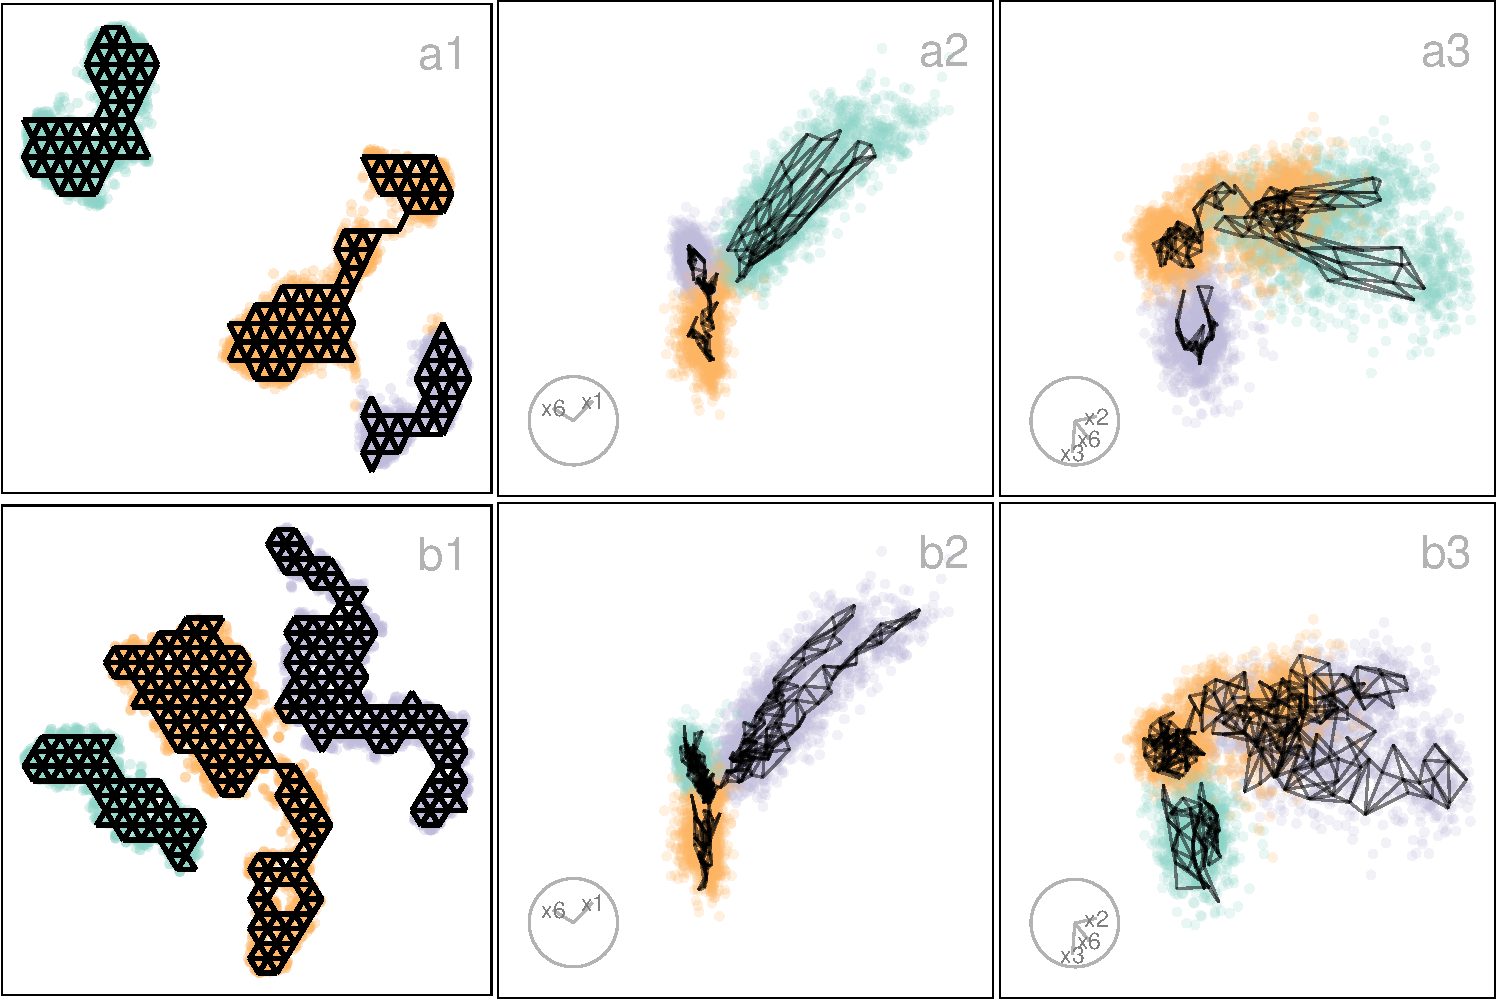
\includegraphics[width=0.8\textwidth,height=\textheight]{paper_files/figure-pdf/fig-model-pbmc-author-proj-1.pdf}

}

\caption{\label{fig-model-pbmc-author-proj}Model in \gD{}, on the layout
a and b, and two views of the fit in projections from \(9\text{-}D\),
for the PBMC3k data (\(n =  2622\) and \(p = 9\)). Layout a shows
three-well separated clusters with big separation, while layout b shows
close clusters. In \(9\text{-}D\), the data shows three clusters with
two of them being close and one separated from the others. This is why
b1, b2, and b3 shows a connected edge between the close clusters, as
proven by Figure~\ref{fig-pbmc-mse} as a reasonable layout. Viewing the
fitted model in \(9\text{-}D\), helps to see some unobserved patterns of
the data: (i) dense points, and (ii) non-linear clusters. Videos of the
langevitour animations are available at
\url{https://youtu.be/0cKX_HG_n0k} and
\url{https://youtu.be/KhJvsRtaX04} respectively.}

\end{figure}%

\subsubsection{Comparison with results of scDEED
recommendations}\label{comparison-with-results-of-scdeed-recommendations}

In the field of single-cell studies, clustering is a common analytical
task used to identify groups of cells with similar expression profiles.
Non-linear dimensional reduction (NLDR) methods are frequently employed
to visualize these clusters and help validate the results. However, it
is well known that the 2D embeddings produced by t-SNE and UMAP may not
accurately reflect the similarities among cell clusters.

To address this challenge, \citet{xia2023} introduces a statistical
method called scDEED, which detects unreliable cell embeddings generated
by \gD{} embedding techniques. scDEED calculates a reliability score for
each cell embedding based on the similarity between the cell's \gD{}
embedding neighbors and its neighbors prior to embedding. By identifying
embeddings with low reliability scores as dubious and those with high
scores as trustworthy, scDEED minimizes the number of questionable cell
embeddings. This approach also provides clear guidance for optimizing
the hyperparameters of an embedding method.

To verify that the \gD{} cell embeddings became better aligned with the
cell types after scDEED's optimization, the Human Peripheral Blood
Mononuclear Cells (PBMC) dataset was used. It contained \(31,021\) cells
with cell type labels, and the gene expression levels were in the unit
of log-transformed UMI count per \(10,000\). They focused on three
sequencing methods (inDrops, DropSeq, and SeqWell) and four common cell
types Cytotoxic T cell, CD4+T cell, CD14+ Monocyte, and B cell.

For illustration purposes, we only selected cells generated with inDrops
(\(n=5858\) cells) and UMAP cell embeddings. Also, \citet{xia2023} used
first \(50\) principal components to generate the UMAP. The objective is
to assess the optimized layout by scDEED, and if it does not accurately
represent the three clusters with small separations of the PBMC dataset,
then select a reasonable \gD{} layout.

\begin{figure}[H]

\centering{

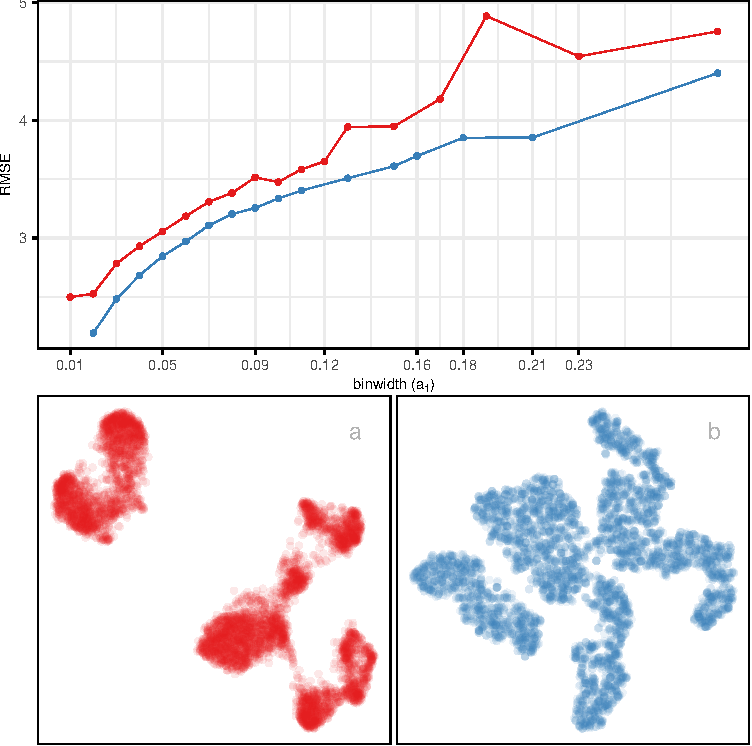
\includegraphics[width=1\textwidth,height=\textheight]{paper_files/figure-pdf/fig-pbmc-mse-umap-1.pdf}

}

\caption{\label{fig-pbmc-mse-umap}Assessing which of the 2 UMAP layouts
with different hyperparameter settings (n\_neighbors: \(30\), min\_dist:
\(0.3\) (red), n\_neighbors: \(80\), min\_dist: \(0.5\) (blue)) on the
PBMC data is the better representation using MSE for varying binwidth
(\(a_1\)). Colour used for the lines and points in the left plot and in
the scatterplots represents UMAP layout (a, b). Layout b is universally
suboptimal. Layout b is the best choice.}

\end{figure}%

\begin{figure}[H]

\centering{

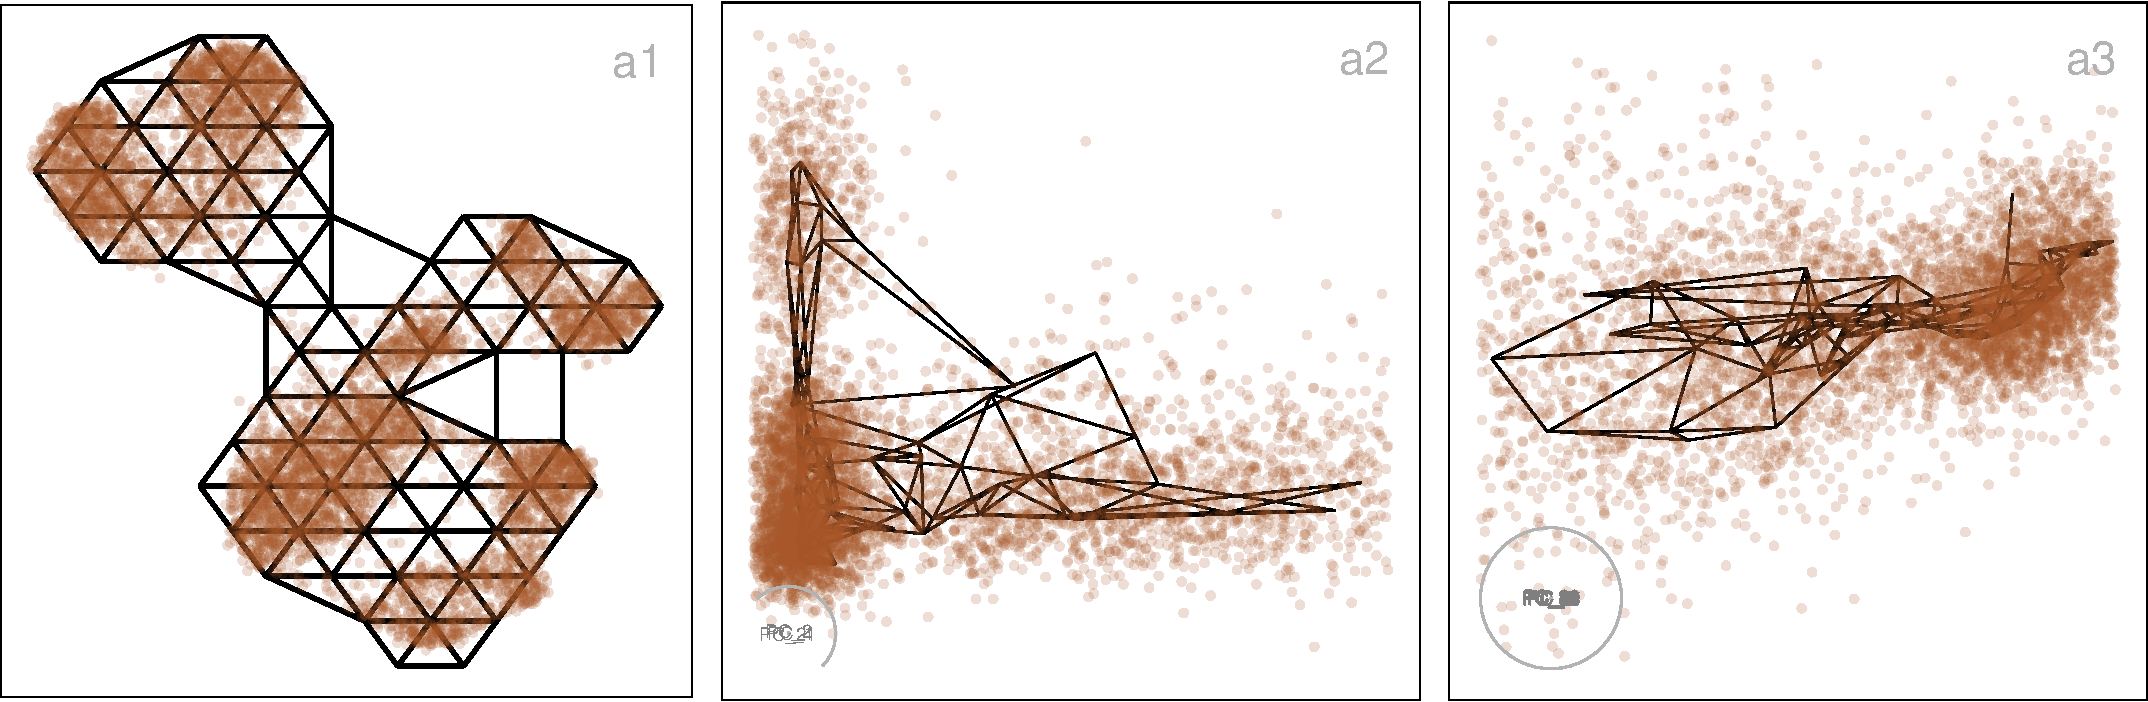
\includegraphics[width=0.8\textwidth,height=\textheight]{paper_files/figure-pdf/fig-model-pbmc-author-proj-scdeed-1.pdf}

}

\caption{\label{fig-model-pbmc-author-proj-scdeed}Model in \gD{}, on the
layout a, and two views of the fit in projections from \(50\text{-}D\),
for the PBMC data (\(n =  5858\) and \(p = 50\)). Layout shows close
clusters. In \(50\text{-}D\), the data shows}

\end{figure}%

\subsection{Hand-written digits}\label{hand-written-digits}

The digit 1 of the MNIST dataset consists of \(7877\) grayscale images
of handwritten digits \citep{lecun2010}. Before further analysis, PCA
was used to preprocess the data, where the first \(10\) principal
components, explaining 83\% of the total variation, were selected. The
objective is to select a reasonable \gD{} layout, representing the
non-linear structure of the digit 1 dataset in \(10\text{-}D\)
(Figure~\ref{fig-mnist-tri-proj} (a)).

\begin{figure}[H]

\centering{

\includegraphics[width=1\textwidth,height=\textheight]{paper_files/figure-pdf/fig-mnist-mse-1.pdf}

}

\caption{\label{fig-mnist-mse}Assessing which of the 5 NLDR layouts on
the MNIST digit 1 data is the better representation using MSE for
varying binwidth (\(a_1\)). Colour used for the lines and points in the
left plot and in the scatterplots represents NLDR layout (a-e). All the
layouts appear to be very similar. Layout c is universally poor. Layouts
a that show two close clusters are universally suboptimal. Layout a is
the best choice.}

\end{figure}%

The MSE for different binwidths (\(a_1\)) using tSNE, UMAP, PHATE,
PaCMAP, and TriMAP with default (hyper-)parameter setting
(Figure~\ref{fig-mnist-mse}) were calculated. It is found that tSNE
(Figure~\ref{fig-mnist-mse} (a)) provide the most reasonable
representation for the digit 1 dataset, showing universally best.
However, \gD{} representation shows a big non-linear cluster and a small
cluster with a small gap (\textbf{?@fig-tsne-best}).

In the case of digit 1 data, there should not be any clusters unless
anomalies exist, indicating different digit 1 patterns. The angle of the
digit 1 images varies along this non-linear clustering structure
(\textbf{?@fig-tsne-best}), while the small cluster contains the digit 1
images with different patterns of the digit 1, unlike the usual
(Figure~\ref{fig-model-error-mnist} (c)). This provides the evidence for
two close clusters.

By visualizing the model generated for tSNE in \(10\text{-}D\) helps to
assess the \gD{} layout. As shown in Figure~\ref{fig-mnist-tri-proj}
(a), the model provides the evidence for the non-linear structure of the
digit 1 data in \(10\text{-}D\). The model shows some quirks. The
model's twisted pattern provides evidence for the \(10\text{-}D\) data
structure, which is not observed by \gD{} layout
(Figure~\ref{fig-mnist-tri-proj} (b)). Furthermore, the presence of long
edges indicates the existence of the small cluster located closely
together (Figure~\ref{fig-mnist-tri-proj} (c)).

\begin{figure}[H]

\centering{

\includegraphics[width=1\textwidth,height=\textheight]{paper_files/figure-pdf/fig-mnist-tri-proj-1.pdf}

}

\caption{\label{fig-mnist-tri-proj}Model in \gD{}, on the layout a and
three views of the fit in projections from \(10\text{-}D\), for the
MNIST digit 1 data (\(n =  7877\) and \(p = 10\)). There is a big
non-linear cluster and a small clusterlocated very close to one corner
of the big cluster. There is a twisted pattern that is hardly visible in
the static plot. Video of the langevitour animation are available at .}

\end{figure}%

\begin{figure}[H]

\centering{

\includegraphics[width=0.8\textwidth,height=\textheight]{paper_files/figure-pdf/fig-model-error-mnist-1.pdf}

}

\caption{\label{fig-model-error-mnist}The \(10\text{-}D\) model error in
layout a of the MNIST digit 1 dataset show a pattern. Most low model
errors are distributed along the big non-linear clutser, while most
large model errors are distributed along the small cluster. Along the
non-linear cluster, the angle of digit 1 changes. Some images have large
errors due to their deviation from the non-linear cluster, which makes
them anomalies. The images associated with large model errors shows
different patterns of digit 1.}

\end{figure}%

\section{Discussion}\label{sec-discussion}

This study makes several important contributions to the field of NLDR.
We have developed an algorithm to evaluate the most useful NLDR method
and (hyper-)parameter choices for creating an accurate \gD{} layout of
high-dimensional data. Our objective is to fit a model for the \gD{}
layout that preserves the relationships between neighboring points and
turns it into a high-dimensional wireframe, which can be overlaid on the
data and visualized using a tour. This approach is defined as
\emph{model-in-data-space}. Viewing a model in the data space is an
ideal way to examine the fit.

The effectiveness of this approach is illustrated through various
examples. For instance, the two-curvy clusters example demonstrates how
the model accurately fits the points, capturing both local and global
structures in high-dimensional space. Our simulation case study further,
five Gaussian cluster example shows that while all observed NLDR methods
preserve the global structure, only tSNE effectively maintains the local
structure, highlighting the specific strengths and quirks of different
methods.

Human behavior often shows a desire for more certainty and a tendency to
prefer well-separated views. This emphasizes the importance of clear and
distinct clusters. For example, in the UMAP layout of the
\textbf{PBMC3k} dataset suggested by \citet{chen2023}, three distant,
well-separated clusters are shown. However, our model reveals that these
clusters are actually close to each other in \pD{}. Additionally, the
model discovers non-uniform data distribution and non-linear structures
within the clusters that are not visible in the UMAP layout,
demonstrating the ability of our model in uncovering hidden data
characteristics.

Evaluating the error or unexplained variance is important for assessing
how well the model fits the data. By examining the error for different
numbers of bins, we found that tSNE with a perplexity of \(30\) provides
a reasonable representation for the \textbf{pbmc} dataset. Connecting
the closest clusters with line segments in the fitted model further
supports the preservation of neighborhood relationships.

The \textbf{digit: 1} example further illustrates the model's ability to
accurately capture non-linear structures and provide additional
information. Key findings include a twisted pattern that compresses the
structure in some projections and long line segments that detect
anomalies.

Predicting new observations in \kD{} is particularly valuable due to the
limitations of some NLDR methods, like tSNE, which don't provide a
straightforward method for prediction. As a result, our approach offers
a solution that capable of generating predicted \kD{} embedding
regardless of the NLDR method employed, effectively addressing this
functional gap.

In conclusion, while our method effectively captures and represents
high-dimensional data structures, further enhancements could involve
introducing approaches to bind the data, indicate line segments beyond
\gD{}, and diagnose the fitted model. These improvements would help in
creating a more accurate representation of the data when \gD{} layout is
inadequate.

\section{Supplementary Materials}\label{supplementary-materials}

Appendix: The appendix includes more details about the hexagonal binning
algorithm (appendix.pdf, Portable Document Format file).

R package \texttt{quollr}: The R package \texttt{quollr} containing
codes to fit, and visualize the model. (need to add quollr .zip file,
GNU zipped tar file)

\section{Acknowledgments}\label{acknowledgments}

These \texttt{R} packages were used for the work: \texttt{tidyverse}
(\citet{hadley2019}), \texttt{png} (\citet{simon2022}), \texttt{Rtsne}
(\citet{jesse2015}), \texttt{umap} (\citet{tomasz2023}),
\texttt{ggplot2} (\citet{hadley2016}), \texttt{patchwork}
(\citet{thomas2024}), \texttt{colorspace} (\citet{achim2020}),
\texttt{langevitour} (\citet{harisson2024}), \texttt{conflicted}
(\citet{hadley2023}), \texttt{reticulate} (\citet{kevin2024}),
\texttt{kableExtra} (\citet{hao2024}). These \texttt{python} packages
were used for the work: \texttt{trimap} (\citet{amid2022}) and
\texttt{pacmap} (\citet{yingfan2021}). The article was created with
\texttt{R} packages \texttt{rticles} (\citet{jjallaire2024}),
\texttt{knitr} (\citet{yihui2014}), and \texttt{rmarkdown}
(\citet{yihui2020}). The project's GitHub repository
(\url{https://github.com/JayaniLakshika/paper-nldr-vis-algorithm})
contains all materials required to reproduce this article.

\section*{References}\label{references}
\addcontentsline{toc}{section}{References}

\renewcommand{\bibsection}{}
\bibliography{bibliography.bib}

\newpage{}





\end{document}
